% `template.tex', a bare-bones example employing the AIAA class.
%
% For a more advanced example that makes use of several third-party
% LaTeX packages, see `advanced_example.tex', but please read the
% Known Problems section of the users manual first.
%
% Typical processing for PostScript (PS) output:
%
%  latex template
%  latex template   (repeat as needed to resolve references)
%
%  xdvi template    (onscreen draft display)
%  dvips template   (postscript)
%  gv template.ps   (onscreen display)
%  lpr template.ps  (hardcopy)
%
% With the above, only Encapsulated PostScript (EPS) images can be used.
%
% Typical processing for Portable Document Format (PDF) output:
%
%  pdflatex template
%  pdflatex template      (repeat as needed to resolve references)
%
%  acroread template.pdf  (onscreen display)
%
% If you have EPS figures, you will need to use the epstopdf script
% to convert them to PDF because PDF is a limmited subset of EPS.
% pdflatex accepts a variety of other image formats such as JPG, TIF,
% PNG, and so forth -- check the documentation for your version.
%
% If you do *not* specify suffixes when using the graphicx package's
% \includegraphics command, latex and pdflatex will automatically select
% the appropriate figure format from those available.  This allows you
% to produce PS and PDF output from the same LaTeX source file.
%
% To generate a large format (e.g., 11"x17") PostScript copy for editing
% purposes, use
%
%  dvips -x 1467 -O -0.65in,0.85in -t tabloid template
%
% For further details and support, read the Users Manual, aiaa.pdf.


% Try to reduce the number of latex support calls from people who
% don't read the included documentation.
%
\typeout{}\typeout{If latex fails to find aiaa-tc, read the README file!}
%


\documentclass[]{aiaa-tc}% insert '[draft]' option to show overfull boxes

 \usepackage{varioref}%  smart page, figure, table, and equation referencing
 \usepackage{wrapfig}%   wrap figures/tables in text (i.e., Di Vinci style)
 \usepackage{threeparttable}% tables with footnotes
 \usepackage{dcolumn}%   decimal-aligned tabular math columns
  \newcolumntype{d}{D{.}{.}{-1}}
 \usepackage{nomencl}%   nomenclature generation via makeindex
  \makeglossary
 % \usepackage{subfigure}% subcaptions for subfigures
 % \usepackage{subfigmat}% matrices of similar subfigures, aka small mulitples
 \usepackage{subcaption}
 \usepackage{fancyvrb}%  extended verbatim environments
  \fvset{fontsize=\footnotesize,xleftmargin=2em}
 \usepackage{lettrine}%  dropped capital letter at beginning of paragraph
 \usepackage[colorlinks]{hyperref}%  hyperlinks [must be loaded after dropping]

 \title{Real-Time Performance Feedback in a \\Manually-Controlled Spacecraft Inspection Task}

 \author{
  John A. Karasinski%
    \thanks{Graduate Student Researcher, Mechanical and Aerospace Engineering, Student Member AIAA.}
  \ and Stephen K. Robinson\thanks{Director – UC Davis Center for Human/Robotics/Vehicle Integration and Performance, Professor – Mechanical and Aerospace Engineering, Member AIAA.}\\
  {\normalsize\itshape
   University of California, Davis, Davis, CA 95616}\\
  \and
  Patrick Handley%
    \thanks{Technical Staff, Member AIAA.}
  \ and Kevin R. Duda\thanks{Principal Aerospace Human Factors Engineer, Member AIAA.}\\
  {\normalsize\itshape
   Charles Stark Draper Laboratory, Cambridge, MA 02139}\\
  % Third C. Author%
  %  \thanks{Job Title, Department, Address, and AIAA Member Grade.}\\
  % {\normalsize\itshape
  % Business or Academic Affiliation, City, Province, Zipcode, Country}
 }

 % Data used by 'handcarry' option if invoked
 \AIAApapernumber{YEAR-NUMBER}
 \AIAAconference{Conference Name, Date, and Location}
 \AIAAcopyright{\AIAAcopyrightD{YEAR}}

 % Define commands to assure consistent treatment throughout document
 \newcommand{\eqnref}[1]{(\ref{#1})}
 \newcommand{\class}[1]{\texttt{#1}}
 \newcommand{\package}[1]{\texttt{#1}}
 \newcommand{\file}[1]{\texttt{#1}}
 \newcommand{\BibTeX}{\textsc{Bib}\TeX}

\begin{document}

\maketitle

\section{Extended Abstract}
\lettrine[nindent=0pt]{W}{e} consider the distinction between guidance --- the information an operator receives about the vehicle's state, and performance feedback --- additional information that an instructor provides while training an operator. Guidance is the process of collecting and applying information for the purpose of generating maneuver commands to control vehicle movements~\cite{draper1965guidance}. In aerospace vehicles, guidance is usually presented to a pilot by visual displays which could include any number of changing numbers, words, lines, or other shapes. In contrast to guidance, feedback should act as an easily-accessible indicator of performance. Guidance already tells the pilot what to do --- feedback should simply inform them if they're following guidance well enough.


While operating a vehicle, well trained operators already know how to fly, but their performance can still be improved with the assistance of an expert providing feedback in real-time. Rather than focusing on the final results of a mission, real-time operator monitoring can produce an assessment of an operator's state and task performance. This, in turn, provides important context for interpreting the operator's actions and is critical for presenting timely and relevant feedback to the operator. We designed an automated flight instructor to provide real-time feedback to a human operator during a simulated Simplified Aid For EVA Rescue (SAFER) flight task. SAFER is a small propulsive jet pack worn during spacewalks for self-rescue~\cite{safer}. We investigate the effect of three variations of an instructor-model performance-feedback strategy on human performance in a novel SAFER inspection task.


A human-in-the-loop simulation was conducted to gather data from 30 subjects (26 males, 4 females), with an average age of $21.9\pm0.7$ years, gathered from undergraduate and graduate students in the UCD school of engineering. Subjects were tasked with flying SAFER to perform an inspection of the International Space Station's (ISS) solar arrays. Subjects started 40 feet away from the solar array, and were asked to close to 30 feet away from the solar array and hold this distance for the remainder of the task. Subjects were then asked to inspect 4 ``damage'' points on the solar array, and were given a guidance display for navigation to the waypoints, see Fig.~\ref{fig:displays}. The flying task included (in priority order):
\begin{enumerate}
\item Holding a specific distance from the solar array (30 feet from the solar array)
\item Minimizing their roll angle (a relative angle of 0 degrees)
\item Navigating to the waypoints as quickly and accurately possible
\end{enumerate}

While performing the flying task, subjects were also asked to respond to a secondary task in the form of a ``comm light''~\cite{crosby1979dual, wickens1986sternberg, hainley2013pilot}. The light would change from a teal color to a blue or a green color every 5 to 7 seconds (at a pseudorandom interval), and the subjects responded by pressing an appropriately labeled button on the joysticks. This secondary task was placed on a separate screen from the flight tasks, and the change in color could not be easily distinguished from the subjects' peripheral vision, requiring the subjects to establish a scan pattern. Response time to this two-choice secondary task was used as an objective measure subject's workload. After each trial, subjects were asked to rate their workload on the Modified Bedford Workload Scale, as a subjective measurement of their workload~\cite{wickens1991processing}. Finally, the subjects also made verbal callouts about their fuel level every time it decreased by 5\% (e.g., 95\%, 90\%, 85\%, ...), which presented us with insight into of their situational awareness.


Under the guiding principle that a superior flight instructor can lead to a better trained student, we seek to answer the following questions:
\begin{enumerate}
\item Can subjects' fully trained performance level be increased with the use of real-time performance feedback?
\item Can subjects' workload be decreased with the use of real-time performance feedback?
\item Can subjects' training time be decreased with the use of real-time performance feedback?
\end{enumerate}

Subjects were placed into one of three groups, and each subject flew a total of 20 trials. Group 1 acted as a control group, and had an analog distance display that read from -10 to 10 feet, and digital displays with one significant figure (e.g., 1, 2, 3...). Group 2 had an analog distance display that read from -5 to 5 feet, and digital display with two significant figures (e.g., 1.2, 2.7, 9.4). Group 3 had the same analog and digital distance displays as Group 1, and experienced real-time feedback in the form of distance and roll displays that changed color. When instantaneous performance fell below a critical value which we chose, the appropriate display changed from green to red. These displays are decoupled, and were activated independently of each other. Group 3 had distance feedback parameter of 1 foot, and a roll feedback parameter of 1.35 degrees, the asymptotic limit of Group 1.


Subject performance can be quantified by taking the mean absolute error between the guidance displays and the subject's actual trajectory, and by the amount of time required to complete the task. Preliminary results suggest Groups 2 and 3 both perform better than the control group on the primary and secondary flight tasks. From the very first trial, subjects in Group 3 were able to perform better than Group 1 could at the end of the experiment, see Fig.~\ref{fig:performance}. This suggests that the real-time performance feedback immediately provided a performance improving effect, even with novice operators. Subjects in the feedback group (Group 3) also reported the lowest levels of workload via their post-trial Modified Bedford Workload scores, see Fig.~\ref{fig:workload}. While both Groups 2 and 3 showed performance improvements over the control group, Group 2's workload was increased, as was their time to complete the task. Group 3 showed even larger performance improvements than Group 2, and also showed lower workload levels and only marginally larger time to complete the task.

\begin{figure}[b!]
  \centering
  \begin{subfigure}{.5\textwidth}
    \centering
    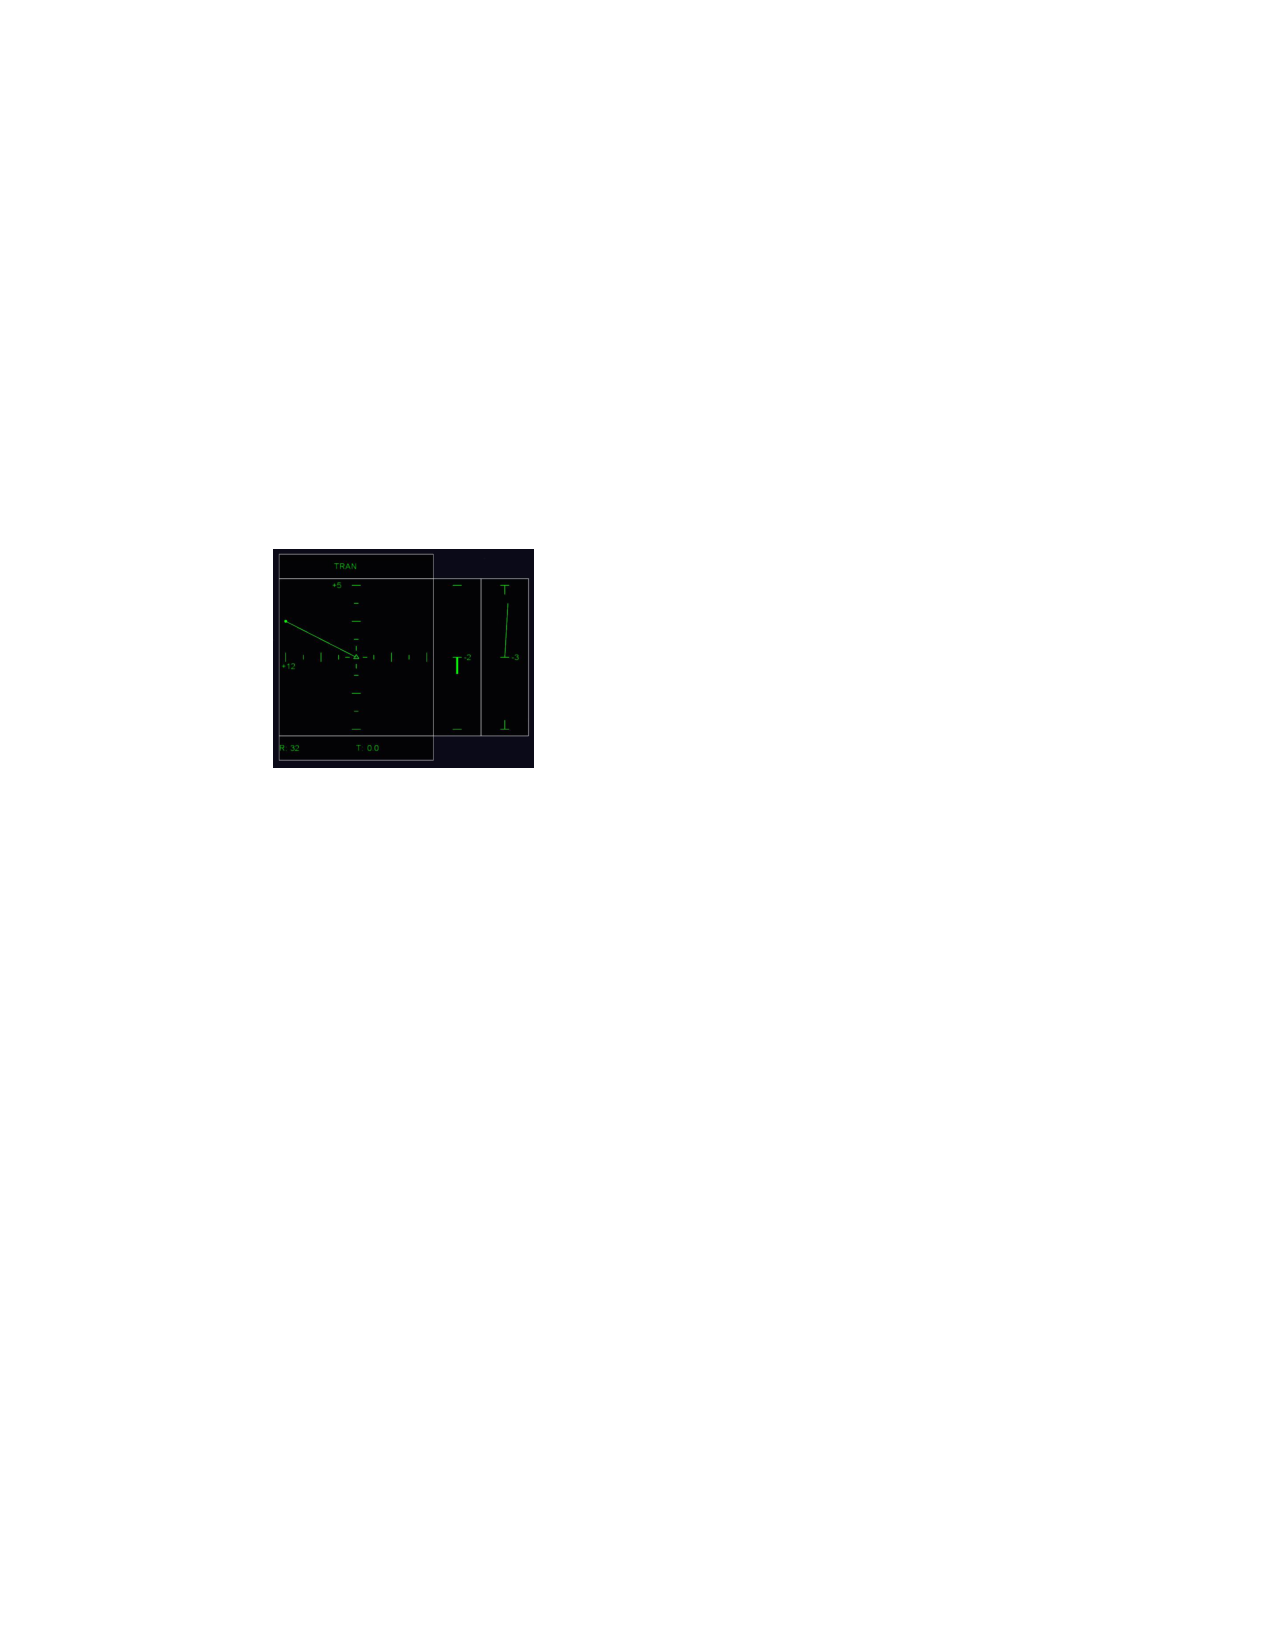
\includegraphics[width=.99\linewidth, page=1]{figs/guidance_full.pdf}
    \caption{Group 1}
    \label{fig:sub1}
  \end{subfigure}%
  \begin{subfigure}{.5\textwidth}
    \centering
    \includegraphics[width=.99\linewidth, page=2]{figs/guidance_full.pdf}
    \caption{Group 2}
    \label{fig:sub2}
  \end{subfigure}\vspace{1em}
  \begin{subfigure}{.5\textwidth}
    \centering
    \includegraphics[width=.99\linewidth, page=3]{figs/guidance_full.pdf}
    \caption{Group 3}
    \label{fig:sub2}
  \end{subfigure}
  \caption{Display differences for all three groups in the same state.}
  \label{fig:displays}
\end{figure}

\begin{figure}[b!]
  \centering
  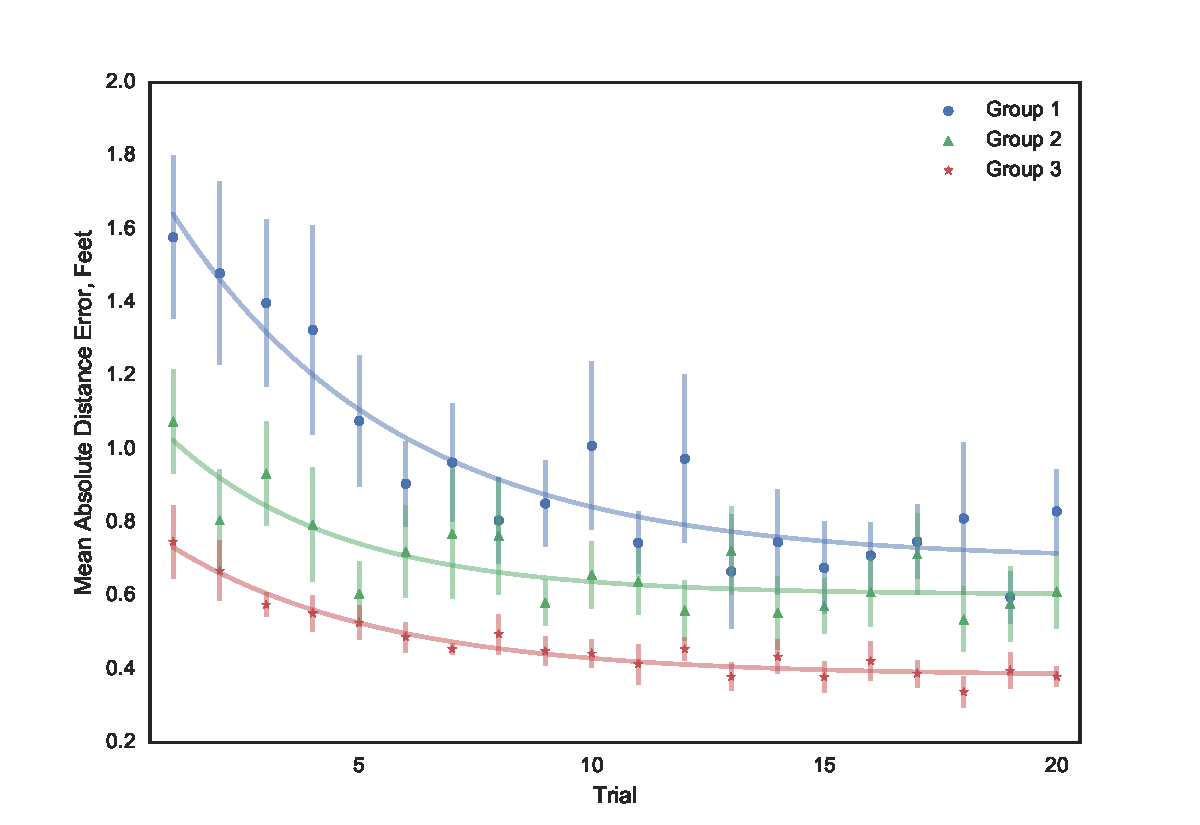
\includegraphics[width=0.8\linewidth]{figs/Group_absDistErr_clean_fit_30.pdf}
  \caption{Mean absolute distance error from the solar array in feet per trial. Data points show the mean; error bars are the standard error of the mean. Lines show exponential fits to the values by trial. All subject group show a large amount of learning during the first half of the experiment, then settle to a steady state value.}
  \label{fig:performance}
\end{figure}

\begin{figure}[b!]
  \centering
  \includegraphics[width=0.8\linewidth]{figs/Group_workload_fit_30.pdf}
  \caption{Mean self reported Modified Bedford Workload Score per trial. Data points show the mean; error bars are the standard error of the mean. Lines show exponential fits to the values by trial. All subjects group initially report the same level of workload, but separate out into individual lines as the experiment continues. Ultimately, Group 2 reports the highest workload, followed by Group 1, and Group 3.}
  \label{fig:workload}
\end{figure}

\section*{Acknowledgments}
This was was supported by the National Space Biomedical Research Intsitute through NASA NCC 9-58, Project HFP03401.

% produces the bibliography section when processed by BibTeX
% \nocite{*}
\bibliography{bibtex_database}
\bibliographystyle{aiaa}

\end{document}

% - Release $Name:  $ -
